\section{Implementation} \label{sec:impl}
In this section, we present the implementation details of the \module and the \cache based on Linux (the guest kernel) and Xen (the hypervisor).

\subsection{\name Module}
\begin{figure}[ht]
\centering
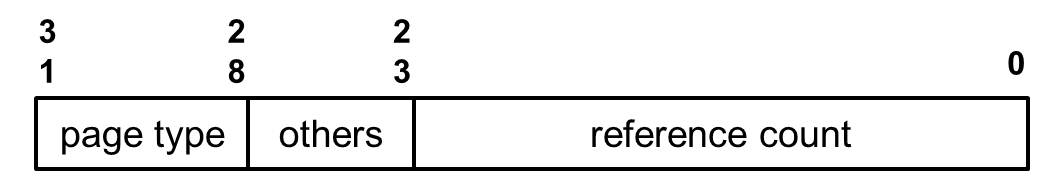
\includegraphics[width=0.45\textwidth]{image/implementation/field-of-page-type-info.jpg} \\
\caption{The layout of the original data structure for page type.}
\label{fig:field-of-page-type-info}
\end{figure}
The first main task of the \module is to extend the existing data structures to support semi-writable page table.
As illustrated in Figure~\ref{fig:field-of-page-type-info}, the data structure for labelling page types is 32bits, i.e., bits 28 - 31 are allocated for page type, bits 23 - 27 is for others (e.g., bit 26 indicate if this page has been validated), and bits (0 - 22) is for reference count.
The existing page types have occupied all page type bits, and there is no extra bit for semi-writable page.
Facing this problem, we do not choose to introducing new data structures, as it would increase the management complexity and result in many modifications of all related management functions.
Instead, we choose to borrowing a bit from \emph{reference count}.
In particular, the \emph{reference count} field has 23 bits, presenting how many references on a page. 
In fact, the system usually does not build so many references on one page. Thus, we borrow the highest bit (bit 22) as the semi-page table bit (as illustrated in Figure~\ref{fig:field-of-semi-type}).
As a consequence, it still supports more than 4 million reference counts, enough for almost all cases. 
Actually, the hypervisor is functioning well in our experiments.

In the page type checking functions (e.g., \_\_get\_page\_type), we only add a few of lines of code to check the semi-writable pages.
When a semi-writable page is involved in the page type update, some validations (e.g., the DMA validations) necessary before may be skipped, simplifying the validation logic in a certain level. 

\begin{figure}[ht]
\centering
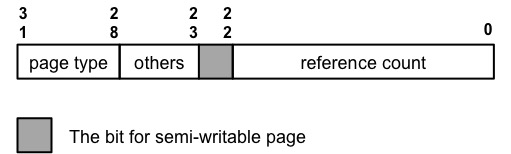
\includegraphics[width=0.45\textwidth]{image/implementation/field-of-semi-type.jpg} \\
\caption{The semi-writable page type support.}
\label{fig:field-of-semi-type}
\end{figure}

\subsection{\name Cache}

In the PV setting, guest OS is required to work in PAE (i.e., Physical Address Extension) mode. As a result, \name maintains three levels of cache pools, each of which is essentially a structured single-linked list caching the guest physical addresses of pages. For the top two levels used for caching PGD (i.e., Page Global Directory) and PMD (i.e., Page Middle Directory), \name obtains the physical addresses directly from their linear addresses. While the bottom PT (i.e., Page Table) is located in the High Memory, the mapping between its linear and physical addresses is not stable. \name acquires the physical addresses of cached PT pages from the corresponding page-info structures.

Every list supports operations of both removal and insertion. Removal exists within the cache allocating function, which fetches a cached page from the top of the list. Insertion is located within the cache freeing function, which inserts a cached page also onto the top. Also, \name maintains two global operation counters, namely num\_in\_use and num\_in\_pool, each logging the invocation times of removal and insertion, respectively. They are required when cache freeing function needs to free cached pages into the buddy system. Every pair of cache allocating and freeing functions is used to hook existing page-table related functions. By this way, whenever OS creates or destroys any process, it always interacts with the caches. Also note that every cache pool and operation counter are shared data resources and their related operation code are critical sections. \name makes use of locks to ensure exclusive resource-access in the multi-processor setting. More specifically, Every level of page-table cache and all its operation counters share a spin lock and irrelevant operations should be removed out of the critical section, especially those that are time-consuming.

\name implements a new system call to provide an interface for users to activate the cache in an on-demand way. In the system call, a global boolean variant is defined, which is initialized as false, indicating that cache is not enabled. And users can assign the variant as true to enable the cache. Anther two user interfaces related to modification of default thresholds and freeing all pages in cache are also implemented through system calls. For the modification, new thresholds of the proportion and total page number are passed as agruments while users can frees all cached pages by resetting a global boolean variant, which is initialized as true.

Within the cache freeing function, a hypercall is implemented with a single-linked list of cached addresses of pages as the parameter. The hypercall is a uniform interface for every level of cache freeing function, simplifying the modifications both to guest OS and Xen. As a reply to the hypercall, Xen mainly zeroes the flag bit of 32-bit field and invokes the important function interface intel\_iommu\_map\_page to create entries in the I/O page tables as well as flush IOTLBs.

